%/*
% * SPDX-FileCopyrightText: 2021 Stefan Begerad <stefan@begerad.de>
% *
% * SPDX-License-Identifier: GPL-3.0-or-later
% */

\begin{frame}{Dede Konzept}
  Die Dede Echtzeit-Karte besteht aus \textbf{drei} Komponenten:
  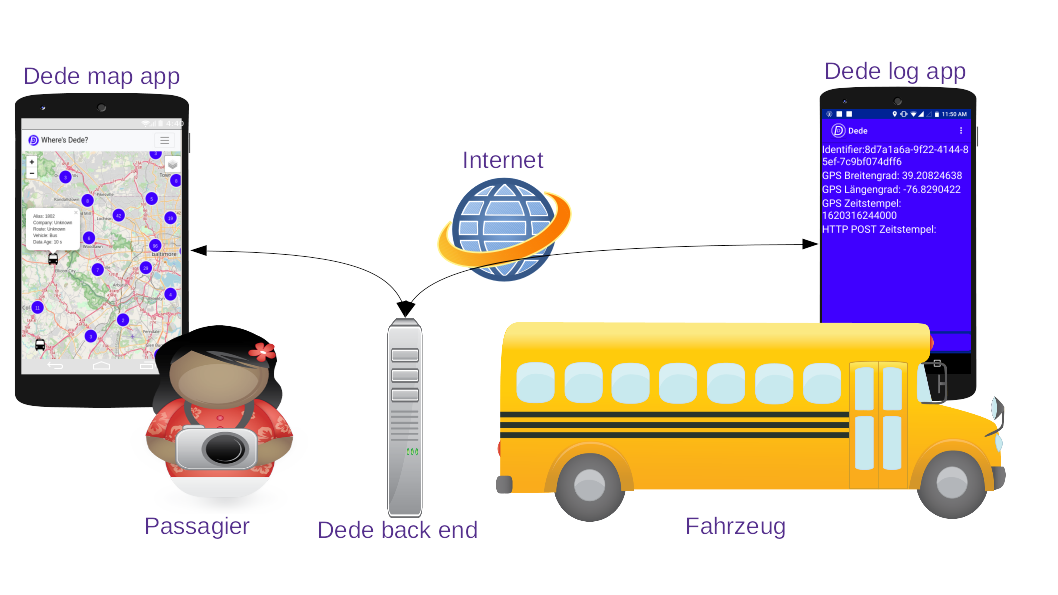
\includegraphics[width=\paperwidth]{dede/dede-concept}
\end{frame}

\begin{frame}{Dede Konzept}
  Der \textbf{Dede Boardrechner} für Smartphones zeichnet die Bewegungsdaten des Fahrzeugs auf und überträgt sie per Internet an den \textbf{Dede-Server}.
  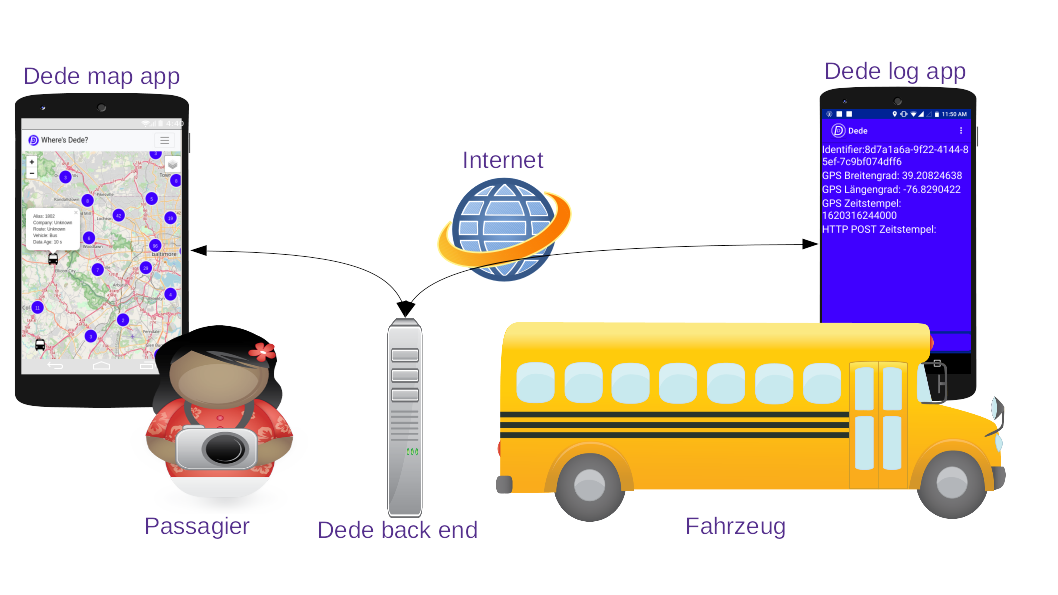
\includegraphics[width=\paperwidth]{dede/dede-concept}
\end{frame}

\begin{frame}{Dede Konzept}
  Der \textbf{Dede-Server} vermittelt zwischen \textbf{Dede Boardrechner} und \textbf{Dede Karte}, so das die Karte \textbf{NICHT} jeden Boardrechner separat abfragen muss.
  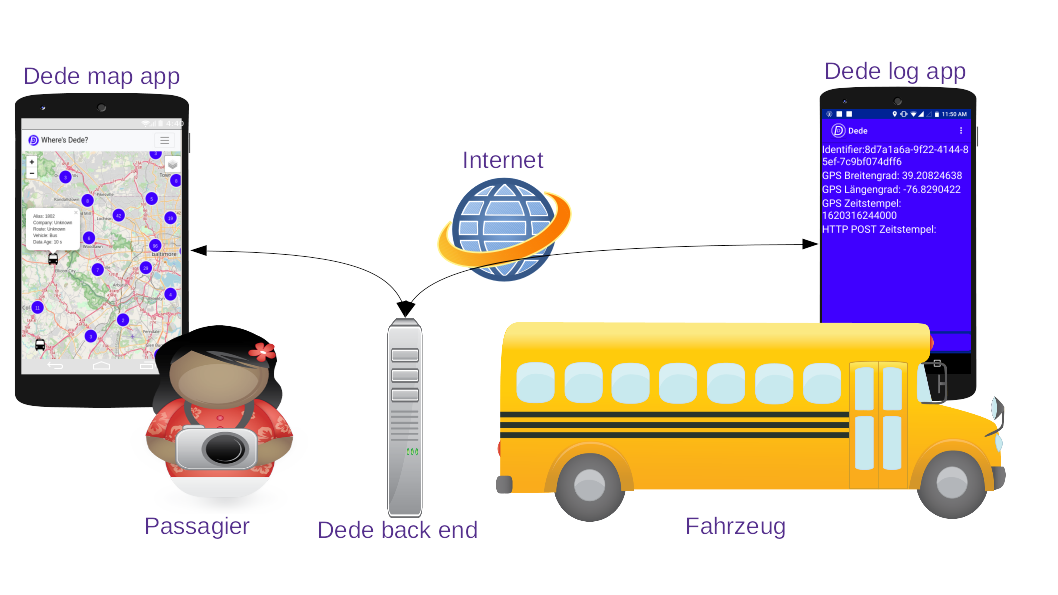
\includegraphics[width=\paperwidth]{dede/dede-concept}
\end{frame}

\begin{frame}{Dede Konzept}
  Die \textbf{Dede Karte} visualisiert die Bewegungdaten auf einer Karte in Echtzeit.
  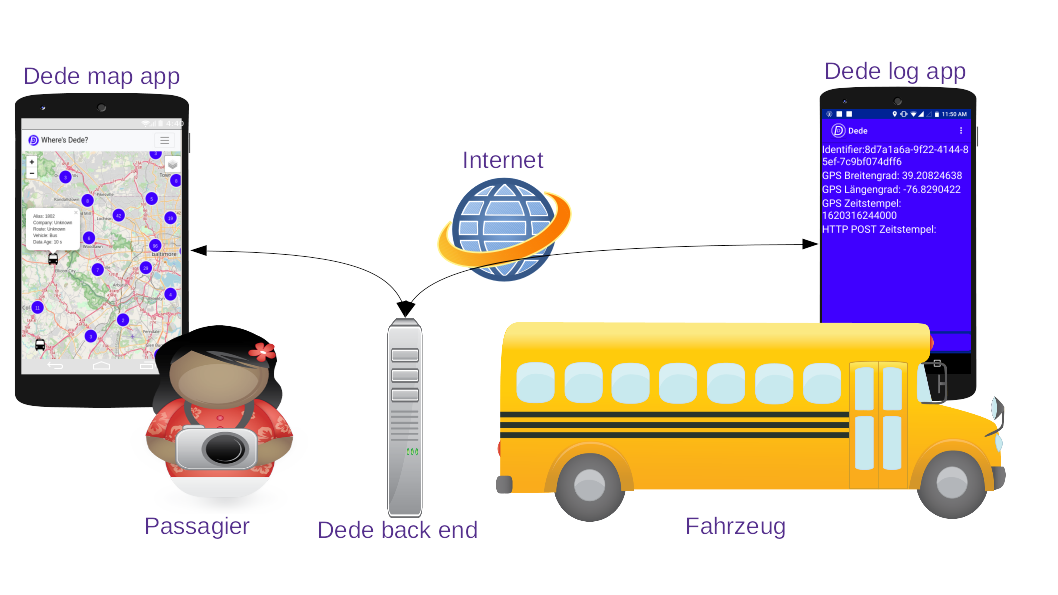
\includegraphics[width=\paperwidth]{dede/dede-concept}
\end{frame}
